\chapter{Preface}

\par
\sputnik is code for calculating a composite material structure. It is composed by two main codes called \macro and
\micro each one design for perfomed coupled calculation with themselves.

\chapter{Homogenization theory}
This chapter is aimed to explain the state of the art on homogenization theory. The main concepts where taken from
\cite{suquet_1985}.

\section{Introduction}

\begin{figure}[h!]
\resizebox{5cm}{!}{
 \documentclass{standalone}

\begin{document}

\begin{tikzpicture}[>=latex,node distance=0pt]

    %\draw [gray!50]  (2,0) -- (13,1) -- (26,6) -- (15,23) -- (1,20) -- cycle;
    \draw [black] plot [smooth cycle] coordinates {(2,0) (13,1) (26,6) (15,23) (1,20)};
    \begin{scope}[yshift = 10 cm,xshift = 8 cm,start chain=going right]
      \draw (0,0) -- (4,0) -- (4,4) -- (0,4) -- cycle;
      \filldraw[fill=black!40!white,draw=black] (2,2) circle (1cm);
    \end{scope}

\end{tikzpicture}

\end{document}


}
\end{figure}

The macroscopic problem :

\[
\begin{cases}
   \text{div } \Sigma =  b\\
   \Sigma = f(E(u))\\
   b.c.
\end{cases}
\]

The microscopic problem :

\[
\begin{cases}
   \text{div } \sigma = 0\\
   \sigma = f(\epsilon(u))\\
   b.c. = g(E , \Sigma) 
\end{cases}
\]

The relation between the maximum size of the r.v.e. ($l$) and the maximum size of the macroscopic 
structure ($L$) as: (\textcolor{blue}{cite the first one in doing this}):

\[
  \eta = \frac{l}{L}
\]
and it will play an important role in this work.

The idea is to try to obtain the same in-situ boundary conditions of the r.v.e. placed on 
the macroscopic structure. This boundary condition are difficult to know a priori so we try to 
approximate them. There are three types of boundary condition that we should consider here : 
\emph{uniform displacement}, \emph{uniform traction} and \emph{periodic}.

%------------------------------------------------------------ 
\subsection{Uniform displacements}
\begin{equation}
u = E \cdot y
\end{equation}

%------------------------------------------------------------ 
\subsection{Uniform tractions}
\begin{equation}
\sigma \cdot \hat{n} = \Sigma
\end{equation}

%------------------------------------------------------------ 
\subsection{Periodic}
Periodic seems to be the most promising b.c. particularly for those cases where $\eta \rightarrow 0$ 
due to the \emph{Saint Venant's Principle}

%------------------------------------------------------------ 
\section{Example}

We are going to focus now on 2D examples to understand the basics on homogenization procedures. \sputnik is 
a 3D code so for obtaining 2D solution we will have to take special care on the boundary conditions of the 
problem.
Let study first the simple case of a composite structure made of an heterogeneous material as shown on figure
\ref{fig_rve_measures}.

The idea is to compare how accurate can be the homogenization procedure under the different boundary 
condition setting. The comparison should be done with some experiment or with a direct calculation, 
this mean to solve the problem numerically considering all the micro-structure details such as the 
one shown on figure \ref{fig_mesh_struc_micro}. 

\begin{figure}[h!]
\fboxsep=0pt
\noindent
%\fbox{%
\begin{minipage}[t]{0.35\linewidth}
\vspace{0pt}
\begin{flushleft}
\resizebox{6cm}{!}{
 \documentclass{standalone}

\begin{document}

\begin{tikzpicture}[>=latex,node distance=0pt,font={\fontsize{50pt}{12}\selectfont}]

% structure
\draw[line width=1.75mm] (0,0) -- (16,0) -- (16,16) -- (0,16) -- cycle;
\foreach \y [count=\n]in {0,4,8,12}{ 
  \foreach \x [count=\n]in {0,4,8,12}{ 
    \begin{scope}[yshift = \y cm,xshift = \x cm,start chain=going right]
      \draw (0,0) -- (4,0) -- (4,4) -- (0,4) -- cycle;
      \filldraw[fill=black!40!white,draw=black] (2,2) circle (1cm);
    \end{scope}
  }
}

% wall lines
\foreach \y [count=\n]in {0,...,15}{ 
 \draw[line width=1.75mm] (-1,\y)-- ++ (1,1) ;
}

% point and arrow for displacement BC
\filldraw[fill=black,draw=black] (16,0) circle (0.3cm);
\draw[-latex,line width=1.75mm] (16,0) -- node[right, xshift=1cm]{$u=d$} (16,-2) ;

%\node (a) at (20,8) {$a=0$} ;

\end{tikzpicture}

\end{document}


}
\end{flushleft}
\end{minipage}
%}%
%\hfill%
%\fbox{%
\begin{minipage}[t]{0.4\linewidth}
\vspace{0pt}
%\begin{flushleft}
Boundary conditions
\[
\begin{cases}
   u_i = 0 \text{ if } x_1 = 0 \text{ for } i=1,2\\
   u_1 = 0, u_2 = d \text{ if } x_1 = L, x_2 = 0\\
   \sigma = 0 \text{ otherwise}
\end{cases}
\]
%\end{flushleft}
\end{minipage}
%}
\caption{Composite material problem to solve.}
\label{fig_rve_measures}
\end{figure}

\begin{figure}[h!]
\resizebox{6cm}{!}{
 \documentclass{standalone}

\begin{document}

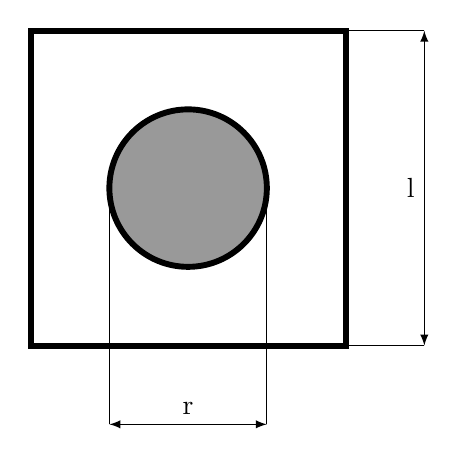
\begin{tikzpicture}

\draw[line width=0.75mm] (0,0) -- (4,0) -- (4,4) -- (0,4) -- cycle;
\filldraw[line width=0.75mm,fill=black!40!white,draw=black] (2,2) circle (1cm);

\draw (3,2) -- (3,-1);
\draw (1,2) -- (1,-1);
\draw[latex-latex] (1,-1) -- node[above] {r} (3,-1);

\draw (4,4) -- (5,4);
\draw (4,0) -- (5,0);
\draw[latex-latex] (5,4) -- node[left] {l} (5,0);

\end{tikzpicture}

\end{document}


}
\caption{r.v.e. that represents the micro-structure}
\label{fig_rve_measures}
\end{figure}


\begin{figure}[h!]
\resizebox{2cm}{!}{
 \documentclass{standalone}

\begin{document}

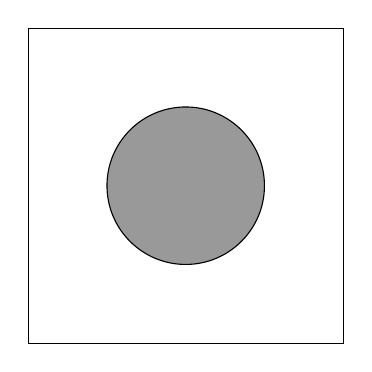
\begin{tikzpicture}

\draw (0,0) -- (4,0) -- (4,4) -- (0,4) -- cycle;
\filldraw[fill=black!40!white,draw=black] (2,2) circle (1cm);

\end{tikzpicture}

\end{document}


}
\end{figure}

\begin{figure}[h!]
\resizebox{5cm}{!}{
 \documentclass{standalone}

\begin{document}

\begin{tikzpicture}[>=latex,node distance=0pt]

\foreach \y [count=\n]in {0,4,8,12}{ 
  \foreach \x [count=\n]in {0,4,8,12}{ 
    \begin{scope}[yshift = \y cm,xshift = \x cm,start chain=going right]
      \draw (0,0) -- (4,0) -- (4,4) -- (0,4) -- cycle;
      \filldraw[fill=black!40!white,draw=black] (2,2) circle (1cm);
    \end{scope}
  }
}

\end{tikzpicture}

\end{document}


}
\end{figure}

\begin{figure}[h!]
  \includegraphics[width=0.5\textwidth]{figures/mesh-struc.pdf}
  \caption{Mesh that represents the hole structure with its micro-structure.}
  \label{fig_mesh_struc_micro}
\end{figure}

\section{Localization and homogenization}

\begin{equation}
E_{ij} = \frac{1}{V}\int_{V}\epsilon_{ij}dy = \langle \epsilon_{ij} \rangle
\end{equation}

\begin{equation}
\Sigma_{ij} = \frac{1}{V}\int_{V}\sigma_{ij}dy = \langle \sigma_{ij} \rangle
\end{equation}

\subsection{Localization}


\subsection{Homogenization}



